\documentclass[a4paper,oneside,12pt, extrafontsizes]{memoir}

\usepackage{graphicx}
\usepackage{verbatim}
\renewcommand{\familydefault}{\sfdefault}
\chapterstyle{demo2}

\title{\emph{Conceptual Modeling Language}\\Specification\\ \small{Version 1.0 (Draft)}}
\author{Quenio Cesar Machado dos Santos\\
\small{Universidade Federal de Santa Catarina}\thanks{
Initially developed as part of the author's Bachelor Technical Report in Computer Sciences}}
\date{July 2017}

\makeatletter
\newcommand{\verbatimfont}[1]{\renewcommand{\verbatim@font}{\ttfamily#1}}
\makeatother

\makeatletter
\renewcommand*{\p@section}{\S\,}
\renewcommand*{\p@subsection}{\S\,}
\makeatother

\begin{document}

\begin{titlingpage}
\maketitle
\end{titlingpage}

\frontmatter

\begin{KeepFromToc}

\clearpage
\tableofcontents

\clearpage
\listoffigures

\clearpage
\listoftables

\end{KeepFromToc}

\mainmatter

\chapter{Introduction}
This document specifies the \emph{Conceptual Modeling Language}, or CML for short.
CML enables the modeling of the information of software systems.
It focuses on modeling the structural aspects of such systems,
having less emphasis on the behavioral aspects.
Using CML,
it is possible to represent the information as understood by the system users,
while disregarding its physical organization as implemented by target languages or technologies.

The CML compiler has:
\begin{itemize}
\item as \emph{input},
source files defined using its own conceptual language (as specified in this document),
which provides an abstract syntax similar to (but less comprehensive than) a combination of UML \cite{uml} and OCL \cite{ocl};
\item and, as \emph{output},
any target languages based on extensible templates,
which may be provided by the compiler's base libraries, by third-party libraries, or even by developers.
\end{itemize}

Section \ref{sec:compiler} will provide an overview of the CML compiler's architecture.
Section \ref{sec:org} describes the organization and notation
used in the remainder of this document.


\chapter{Compiler}
\label{ch:compiler}
The CML compiler's overall architecture follows the standard compiler design literature \cite{torben}. An overview diagram of the architecture is shown in figure \ref{fig:overview}.

\begin{figure}
\centering
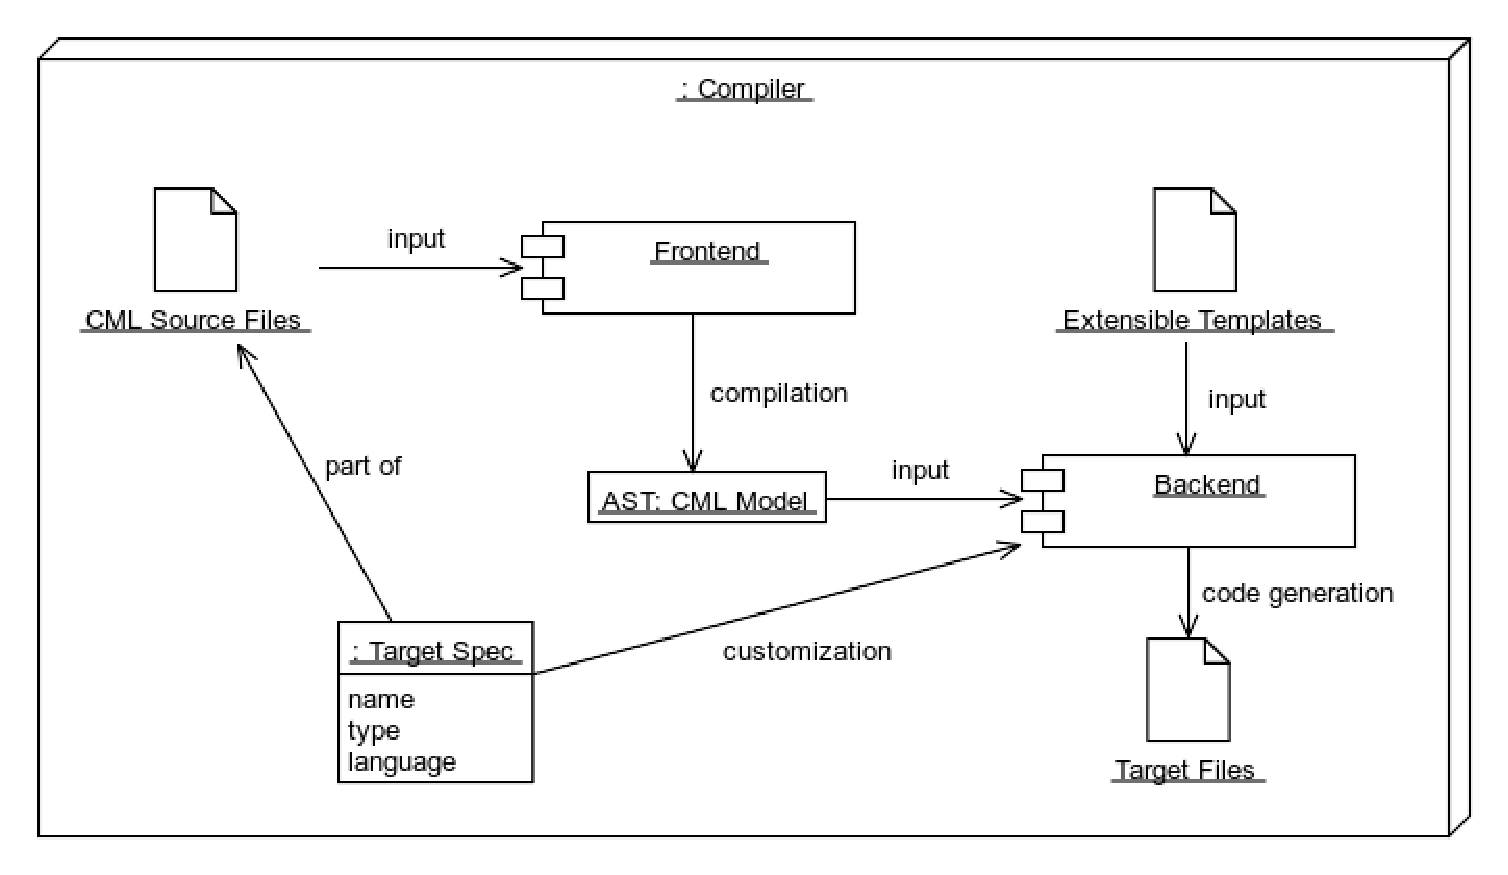
\includegraphics[width=\textwidth]{compiler/figure-overview}
\caption{An architectural overview of the CML compiler.}
\label{fig:overview}
\end{figure}

The two main components of the compiler,
and the artifacts they work with,
are presented in the next subsections.


\chapter{Concepts}

\begin{figure}
\verbatimfont{\small}
\begin{framed}
\verbatiminput{grammar/Concepts.txt}
\end{framed}
\caption{Concept Declaration Syntax}
\label{fig:concept-syntax}
\end{figure}

\section{Properties}\label{sec:properties}

\begin{figure}
\verbatimfont{\small}
\begin{framed}
\verbatiminput{grammar/Properties.txt}
\end{framed}
\caption{Properties Declaration Syntax}
\label{fig:properties-syntax}
\end{figure}

\section{Inheritance}\label{sec:inheritance}


\section{Properties}
\label{sec:properties}
\begin{definition}
A \emph{property} in CML may hold values of primitive types,
in which case they correspond to \emph{attributes}
on the ER \cite{er} and UML \cite{uml} metamodels;
or they may hold references (or collections of references)
linking to instances of other \emph{concepts},
in which case they correspond to a \emph{relationship} on the ER metamodel,
and to \emph{associations} on the UML metamodel.
\end{definition}

\begin{examples}
Figure \ref{fig:ex:properties} presents some examples of \emph{properties} declared in CML.
As shown in the examples,
a \emph{property} may be an \emph{attribute} (\ref{ch:attributes})
of a \emph{primitive type} (\ref{sec:primitive-types}),
or represent the role/end of an \emph{association} (\ref{ch:associations}).
\end{examples}

\begin{figure}
\verbatimfont{\small}
\begin{framed}
\verbatiminput{examples/properties.cml}
\end{framed}
\caption{Property Examples}
\label{fig:ex:properties}
\end{figure}

\begin{concrete-syntax}
Figure \ref{fig:stx:property} specifies the syntax used
to declare a \emph{property}.
The NAME is followed by a \emph{typeDeclaration}
(\ref{sec:primitive-types} and \ref{sec:collection-types}).
Optionally, an \emph{expression} (\ref{ch:expressions}) may be specified
in order to set the initial value.
\end{concrete-syntax}

\begin{figure}
\verbatimfont{\small}
\begin{framed}
\verbatiminput{grammar/Properties.txt}
\end{framed}
\caption{Property Declaration Syntax}
\label{fig:stx:property}
\end{figure}

\begin{abstract-syntax}
Figure \ref{fig:meta:property} presents the \emph{property} metamodel
in an EMOF \cite{mof} class diagram,
and figure \ref{fig:ast:property} specifies
the transformation
from the \emph{property} concrete syntax to its abstract syntax.
For each \emph{property} parsed by the compiler,
an instance of the \emph{Property} class will be created,
and its properties will be assigned
according to parsed information:

\begin{itemize}

\item \emph{name}:
assigned with the value of the terminal node NAME.

\item \emph{type}:
if \emph{typeDeclaration} is provided,
\emph{type} is set with the instance of the \emph{Type} class
matching the \emph{typeDeclaration}.

\item \emph{expression}:
if \emph{expression} is provided,
it contains the instance of the \emph{Expression} class
matching the parsed \emph{expression}.

\end{itemize}
\end{abstract-syntax}

\begin{figure}
\verbatimfont{\small}
\begin{framed}
\verbatiminput{ast/property.lsl}
\end{framed}
\caption{Property AST Instantiation}
\label{fig:ast:property}
\end{figure}


\section{Generalization/Specialization}
\label{sec:generalization}
\begin{definition}
A \emph{concept} in CML may specialize another one,
which is the same as saying that a \emph{concept} is generalized by another one.
In the UML \cite{uml} metamodel,
this generalization/specialization relationship between \emph{classes}
is known as \emph{generalization}, which is the name of the metaclass in the metamodel.
The original version of the ER \cite{er} metamodel lacked this kind of relationship.
\end{definition}

\begin{figure}
\verbatimfont{\small}
\lstinputlisting[language=cml]{examples/generalization.cml}
\caption{Generalization Examples}
\label{fig:ex:concepts}
\end{figure}


\section{Abstract Concepts}
\label{sec:abstract}

\chapter{Attributes}
\begin{definition}
In CML, \emph{attributes} are \emph{properties} (\ref{sec:properties})
of \emph{primitive types} (\ref{sec:primitive-types}).
They correspond to the \emph{Attribute} metaclass 
in the ER \cite{er} and UML \cite{uml} metamodels.
\emph{Attributes} serve as a \emph{slot} to hold a value of 
the specified \emph{primitive type}.
An initial value may be specified as an \emph{expression} (\ref{ch:expressions}).
An \emph{attribute}'s value may also be constantly
derived from an \emph{expression} (not only initially),
in which case it is called a \emph{derived attribute} (\ref{sec:derived-attributes}).
While initial values are only set when a \emph{concept} (\ref{ch:concepts})
is instantiated,
the value of \emph{derived attributes} are always evaluated 
from the given \emph{expression},
and they cannot be set any other way.
\end{definition}

\begin{examples}
Figure \ref{fig:ex:attributes} presents some examples of \emph{attributes} declared in CML.
As shown,
the attribute \textbf{a} is a regular attribute definition 
that specifies the \emph{primitive type} (\ref{sec:primitive-types})
of the values that can be held by the \emph{attribute}'s slot.
The attribute \textbf{b} is an example showing how an \emph{attribute}
can be defined with an initial value.
As shown by the attribute \textbf{c}, 
an attribute may be derived from an \emph{expression}
that refers to other \emph{attributes}.
In order to differentiate \emph{attributes} with initial values
from \emph{derived attributes},
a forward slash (``/'') prefixes the name of the latter.
Attributes \textbf{d} and \textbf{e} are examples
where the type of the attribute,
instead of being specified,
is inferred from the given \emph{expression}.
Type inference is possible for both slot-based \emph{attributes}
and \emph{derived attributes} that provide an \emph{expression}.
\end{examples}

\begin{figure}
\verbatimfont{\small}
\lstinputlisting[language=cml]{examples/attributes.cml}
\caption{Examples of Attributes}
\label{fig:ex:attributes}
\end{figure}


\chapter{Associations}

\section{Unidirectional Associations}\label{sec:assoc-unidir}

\section{Bidirectional Associations}\label{sec:assoc-bidir}

\section{Collection Types}\label{sec:collection-types}


\chapter{Expressions}

\chapter{Targets}
\label{ch:targets}

\chapter{Modules and Libraries}

\appendix

\chapter{Concrete Syntax (Grammar)}
\clearpage
\section{ANTLR Grammar}

\begin{framed}
\verbatimfont{\small}
\begin{verbatim}
// Compilation Units:
\end{verbatim}
\verbatiminput{grammar/CompilationUnits.txt}
\begin{verbatim}
// Concept Declarations:
\end{verbatim}
\verbatiminput{grammar/Concepts.txt}
\begin{verbatim}
// Property Declarations:
\end{verbatim}
\verbatiminput{grammar/Properties.txt}
\begin{verbatim}
// Type Declarations:
\end{verbatim}
\verbatiminput{grammar/Types.txt}
\begin{verbatim}
// Target Declarations:
\end{verbatim}
\verbatiminput{grammar/Targets.txt}
\begin{verbatim}
// Names:
\end{verbatim}
\verbatiminput{grammar/Names.txt}
\begin{verbatim}
// Literals:
\end{verbatim}
\verbatiminput{grammar/Literals.txt}
\verbatiminput{grammar/Ignored.txt}
\end{framed}


\chapter{Abstract Syntax (Metamodel)}
\input{metamodel.tex}

\chapter{Abstract Syntax Tree (Instantiation)}
\input{ast.tex}

\backmatter

\bibliographystyle{plain}
\bibliography{references}

\end{document}
